\subsection{Reduced\-Image  Class Reference}
\label{class_reducedimage}\index{ReducedImage@{Reduced\-Image}}
a handle to access data associated to an image: the fits file, the catalog, the dead and satur frames, and a set of 'scalars' such as seeing, saturation level \&co. 


{\tt \#include $<$reducedimage.h$>$}

Inheritance diagram for Reduced\-Image::\begin{figure}[H]
\begin{center}
\leavevmode
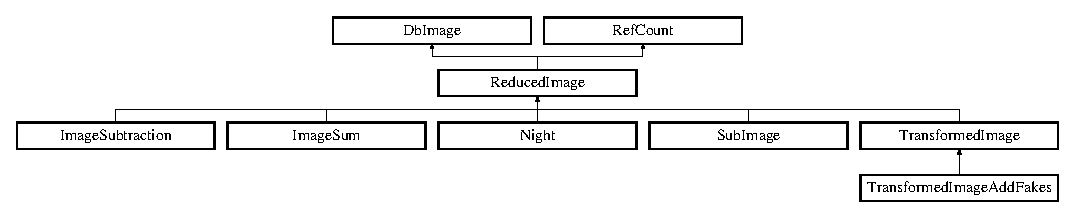
\includegraphics[height=2.47514cm]{class_reducedimage}
\end{center}
\end{figure}
\subsubsection*{Public Methods}
\begin{CompactItemize}
\item 
\index{ReducedImage@{ReducedImage}!ReducedImage@{Reduced\-Image}}\index{ReducedImage@{ReducedImage}!ReducedImage@{Reduced\-Image}}
{\bf Reduced\-Image} ()\label{class_reducedimage_a0}

\item 
\index{ReducedImage@{ReducedImage}!ReducedImage@{Reduced\-Image}}\index{ReducedImage@{ReducedImage}!ReducedImage@{Reduced\-Image}}
{\bf Reduced\-Image} (const {\bf Db\-Image} \&)\label{class_reducedimage_a1}

\item 
\index{ReducedImage@{ReducedImage}!ReducedImage@{Reduced\-Image}}\index{ReducedImage@{ReducedImage}!ReducedImage@{Reduced\-Image}}
{\bf Reduced\-Image} (const string \&Name)\label{class_reducedimage_a2}

\item 
\index{HasImage@{HasImage}!ReducedImage@{Reduced\-Image}}\index{ReducedImage@{ReducedImage}!HasImage@{Has\-Image}}
bool {\bf Has\-Image} () const\label{class_reducedimage_a3}

\item 
\index{HasBack@{HasBack}!ReducedImage@{Reduced\-Image}}\index{ReducedImage@{ReducedImage}!HasBack@{Has\-Back}}
bool {\bf Has\-Back} () const\label{class_reducedimage_a4}

\item 
\index{HasMiniBack@{HasMiniBack}!ReducedImage@{Reduced\-Image}}\index{ReducedImage@{ReducedImage}!HasMiniBack@{Has\-Mini\-Back}}
bool {\bf Has\-Mini\-Back} () const\label{class_reducedimage_a5}

\item 
\index{HasCatalog@{HasCatalog}!ReducedImage@{Reduced\-Image}}\index{ReducedImage@{ReducedImage}!HasCatalog@{Has\-Catalog}}
bool {\bf Has\-Catalog} () const\label{class_reducedimage_a6}

\item 
\index{HasDead@{HasDead}!ReducedImage@{Reduced\-Image}}\index{ReducedImage@{ReducedImage}!HasDead@{Has\-Dead}}
bool {\bf Has\-Dead} () const\label{class_reducedimage_a7}

\item 
\index{HasFlat@{HasFlat}!ReducedImage@{Reduced\-Image}}\index{ReducedImage@{ReducedImage}!HasFlat@{Has\-Flat}}
bool {\bf Has\-Flat} () const\label{class_reducedimage_a8}

\item 
\index{HasSatur@{HasSatur}!ReducedImage@{Reduced\-Image}}\index{ReducedImage@{ReducedImage}!HasSatur@{Has\-Satur}}
bool {\bf Has\-Satur} () const\label{class_reducedimage_a9}

\item 
\index{HasCosmic@{HasCosmic}!ReducedImage@{Reduced\-Image}}\index{ReducedImage@{ReducedImage}!HasCosmic@{Has\-Cosmic}}
bool {\bf Has\-Cosmic} () const\label{class_reducedimage_a10}

\item 
\index{HasSatellite@{HasSatellite}!ReducedImage@{Reduced\-Image}}\index{ReducedImage@{ReducedImage}!HasSatellite@{Has\-Satellite}}
bool {\bf Has\-Satellite} () const\label{class_reducedimage_a11}

\item 
\index{HasWeight@{HasWeight}!ReducedImage@{Reduced\-Image}}\index{ReducedImage@{ReducedImage}!HasWeight@{Has\-Weight}}
bool {\bf Has\-Weight} () const\label{class_reducedimage_a12}

\item 
\index{HasBad@{HasBad}!ReducedImage@{Reduced\-Image}}\index{ReducedImage@{ReducedImage}!HasBad@{Has\-Bad}}
bool {\bf Has\-Bad} () const\label{class_reducedimage_a13}

\item 
\index{FitsName@{FitsName}!ReducedImage@{Reduced\-Image}}\index{ReducedImage@{ReducedImage}!FitsName@{Fits\-Name}}
string {\bf Fits\-Name} () const\label{class_reducedimage_a14}

\begin{CompactList}\small\item\em not const because it may actually compute the image and other things (for derived class).\item\end{CompactList}\item 
\index{MakeFits@{MakeFits}!ReducedImage@{Reduced\-Image}}\index{ReducedImage@{ReducedImage}!MakeFits@{Make\-Fits}}
virtual bool {\bf Make\-Fits} ()\label{class_reducedimage_a15}

\begin{CompactList}\small\item\em produce fits image.\item\end{CompactList}\item 
\index{CatalogName@{CatalogName}!ReducedImage@{Reduced\-Image}}\index{ReducedImage@{ReducedImage}!CatalogName@{Catalog\-Name}}
string {\bf Catalog\-Name} () const\label{class_reducedimage_a16}

\item 
\index{FillSExtractorData@{FillSExtractorData}!ReducedImage@{Reduced\-Image}}\index{ReducedImage@{ReducedImage}!FillSExtractorData@{Fill\-SExtractor\-Data}}
void {\bf Fill\-SExtractor\-Data} (For\-SExtractor \&data, bool fond\_\-deja\_\-soustrait, bool sauver\_\-fond, bool use\_\-sigma\_\-header)\label{class_reducedimage_a17}

\item 
\index{RecoverBack@{RecoverBack}!ReducedImage@{Reduced\-Image}}\index{ReducedImage@{ReducedImage}!RecoverBack@{Recover\-Back}}
bool {\bf Recover\-Back} (bool add\_\-to\_\-im)\label{class_reducedimage_a18}

\item 
\index{ReAddBackground_and_ResetKeys@{ReAddBackground\_\-and\_\-ResetKeys}!ReducedImage@{Reduced\-Image}}\index{ReducedImage@{ReducedImage}!ReAddBackground_and_ResetKeys@{Re\-Add\-Background\_\-and\_\-Reset\-Keys}}
bool {\bf Re\-Add\-Background\_\-and\_\-Reset\-Keys} ()\label{class_reducedimage_a19}

\item 
\index{MakeCatalog@{MakeCatalog}!ReducedImage@{Reduced\-Image}}\index{ReducedImage@{ReducedImage}!MakeCatalog@{Make\-Catalog}}
bool {\bf Make\-Catalog} (bool redo\_\-from\_\-beg, bool overwrite, bool savemasksat, bool pas\_\-sub\_\-fond, bool use\_\-sigma\_\-header)\label{class_reducedimage_a20}

\item 
\index{MakeCatalog@{MakeCatalog}!ReducedImage@{Reduced\-Image}}\index{ReducedImage@{ReducedImage}!MakeCatalog@{Make\-Catalog}}
virtual bool {\bf Make\-Catalog} ()\label{class_reducedimage_a21}

\begin{CompactList}\small\item\em Produce the Saturated stars pixels mask, subtract the image background, detect with the SExtractor computed sigma. search the cosmics, and update catalog and weight for cosmics. No free coffee.\item\end{CompactList}\item 
\index{MakeCatalog_ImageBizarre@{MakeCatalog\_\-ImageBizarre}!ReducedImage@{Reduced\-Image}}\index{ReducedImage@{ReducedImage}!MakeCatalog_ImageBizarre@{Make\-Catalog\_\-Image\-Bizarre}}
bool {\bf Make\-Catalog\_\-Image\-Bizarre} ()\label{class_reducedimage_a22}

\begin{CompactList}\small\item\em {\bf Make\-Catalog\_\-Image\-Bizarre}() {\rm (p.\,\pageref{class_reducedimage_a22})} is for sum-images, or convolved images, for which we do not want to subtract the background map, nor computing the saturated pixels map, and for which we provide the value of the sigmabackground. overwrite is set to true.\item\end{CompactList}\item 
\index{MakeSatur@{MakeSatur}!ReducedImage@{Reduced\-Image}}\index{ReducedImage@{ReducedImage}!MakeSatur@{Make\-Satur}}
virtual bool {\bf Make\-Satur} ()\label{class_reducedimage_a23}

\begin{CompactList}\small\item\em produce satur image.\item\end{CompactList}\item 
\index{MakeDead@{MakeDead}!ReducedImage@{Reduced\-Image}}\index{ReducedImage@{ReducedImage}!MakeDead@{Make\-Dead}}
virtual bool {\bf Make\-Dead} ()\label{class_reducedimage_a24}

\begin{CompactList}\small\item\em produce dead image.\item\end{CompactList}\item 
\index{FlagCosmicsInCatalog@{FlagCosmicsInCatalog}!ReducedImage@{Reduced\-Image}}\index{ReducedImage@{ReducedImage}!FlagCosmicsInCatalog@{Flag\-Cosmics\-In\-Catalog}}
void {\bf Flag\-Cosmics\-In\-Catalog} (const {\bf Image} \&Cosmic\-Image, const double dist=2)\label{class_reducedimage_a25}

\item 
\index{MakeCosmic@{MakeCosmic}!ReducedImage@{Reduced\-Image}}\index{ReducedImage@{ReducedImage}!MakeCosmic@{Make\-Cosmic}}
virtual bool {\bf Make\-Cosmic} ()\label{class_reducedimage_a26}

\begin{CompactList}\small\item\em produce cosmic image.\item\end{CompactList}\item 
\index{MakeSatellite@{MakeSatellite}!ReducedImage@{Reduced\-Image}}\index{ReducedImage@{ReducedImage}!MakeSatellite@{Make\-Satellite}}
virtual bool {\bf Make\-Satellite} ()\label{class_reducedimage_a27}

\begin{CompactList}\small\item\em produce satellite image.\item\end{CompactList}\item 
\index{IsToadsWeight@{IsToadsWeight}!ReducedImage@{Reduced\-Image}}\index{ReducedImage@{ReducedImage}!IsToadsWeight@{Is\-Toads\-Weight}}
bool {\bf Is\-Toads\-Weight} ()\label{class_reducedimage_a28}

\begin{CompactList}\small\item\em produce weight image.\item\end{CompactList}\item 
\index{MakeWeight@{MakeWeight}!ReducedImage@{Reduced\-Image}}\index{ReducedImage@{ReducedImage}!MakeWeight@{Make\-Weight}}
virtual bool {\bf Make\-Weight} ()\label{class_reducedimage_a29}

\item 
\index{MakeBad@{MakeBad}!ReducedImage@{Reduced\-Image}}\index{ReducedImage@{ReducedImage}!MakeBad@{Make\-Bad}}
virtual bool {\bf Make\-Bad} ()\label{class_reducedimage_a30}

\begin{CompactList}\small\item\em produce bad pixel image.\item\end{CompactList}\item 
\index{ActuallyReduced@{ActuallyReduced}!ReducedImage@{Reduced\-Image}}\index{ReducedImage@{ReducedImage}!ActuallyReduced@{Actually\-Reduced}}
bool {\bf Actually\-Reduced} () const\label{class_reducedimage_a31}

\begin{CompactList}\small\item\em returns if both fits image and catalog file exist.\item\end{CompactList}\item 
\index{Execute@{Execute}!ReducedImage@{Reduced\-Image}}\index{ReducedImage@{ReducedImage}!Execute@{Execute}}
bool {\bf Execute} (const int To\-Do)\label{class_reducedimage_a32}

\begin{CompactList}\small\item\em shorthand call for Make\{Fits,Catalog,Dead,Satur\}. To\-Do may conveniently be contructed using predefined tags Do\-Fits Do\-Catalog Do\-Dead Do\-Satur.\item\end{CompactList}\item 
\index{TypeName@{TypeName}!ReducedImage@{Reduced\-Image}}\index{ReducedImage@{ReducedImage}!TypeName@{Type\-Name}}
string {\bf Type\-Name} () const\label{class_reducedimage_a33}

\item 
\index{SetTypeName@{SetTypeName}!ReducedImage@{Reduced\-Image}}\index{ReducedImage@{ReducedImage}!SetTypeName@{Set\-Type\-Name}}
bool {\bf Set\-Type\-Name} (const string \&Type\-Name)\label{class_reducedimage_a34}

\item 
\index{TypeFileName@{TypeFileName}!ReducedImage@{Reduced\-Image}}\index{ReducedImage@{ReducedImage}!TypeFileName@{Type\-File\-Name}}
string {\bf Type\-File\-Name} () const\label{class_reducedimage_a35}

\item 
\index{dump@{dump}!ReducedImage@{Reduced\-Image}}\index{ReducedImage@{ReducedImage}!dump@{dump}}
virtual void {\bf dump} (ostream \&s=cout) const\label{class_reducedimage_a36}

\begin{CompactList}\small\item\em dumps basic info.\item\end{CompactList}\item 
\index{XSize@{XSize}!ReducedImage@{Reduced\-Image}}\index{ReducedImage@{ReducedImage}!XSize@{XSize}}
int {\bf XSize} () const\label{class_reducedimage_a37}

\begin{CompactList}\small\item\em size in x-axis.\item\end{CompactList}\item 
\index{YSize@{YSize}!ReducedImage@{Reduced\-Image}}\index{ReducedImage@{ReducedImage}!YSize@{YSize}}
int {\bf YSize} () const\label{class_reducedimage_a38}

\begin{CompactList}\small\item\em size in y-axis.\item\end{CompactList}\item 
\index{Seeing@{Seeing}!ReducedImage@{Reduced\-Image}}\index{ReducedImage@{ReducedImage}!Seeing@{Seeing}}
double {\bf Seeing} () const\label{class_reducedimage_a39}

\begin{CompactList}\small\item\em basic seeing.\item\end{CompactList}\item 
\index{RemoveSeeing@{RemoveSeeing}!ReducedImage@{Reduced\-Image}}\index{ReducedImage@{ReducedImage}!RemoveSeeing@{Remove\-Seeing}}
void {\bf Remove\-Seeing} ()\label{class_reducedimage_a40}

\item 
\index{SetSeeing@{SetSeeing}!ReducedImage@{Reduced\-Image}}\index{ReducedImage@{ReducedImage}!SetSeeing@{Set\-Seeing}}
bool {\bf Set\-Seeing} (const double \&Value, const string Comment=\char`\"{}\char`\"{})\label{class_reducedimage_a41}

\item 
\index{GetPsfShapeParams@{GetPsfShapeParams}!ReducedImage@{Reduced\-Image}}\index{ReducedImage@{ReducedImage}!GetPsfShapeParams@{Get\-Psf\-Shape\-Params}}
bool {\bf Get\-Psf\-Shape\-Params} (double \&Sigma\-X, double \&Sigma\-Y, double \&Theta\-XY) const\label{class_reducedimage_a42}

\begin{CompactList}\small\item\em basic PSF shape parameters.\item\end{CompactList}\item 
\index{SetPsfShapeParams@{SetPsfShapeParams}!ReducedImage@{Reduced\-Image}}\index{ReducedImage@{ReducedImage}!SetPsfShapeParams@{Set\-Psf\-Shape\-Params}}
bool {\bf Set\-Psf\-Shape\-Params} (const double \&Sigma\-X, const double \&Sigma\-Y, const double \&Theta\-XY, const string Comment=\char`\"{}\char`\"{})\label{class_reducedimage_a43}

\item 
\index{GetRaDecEpoch@{GetRaDecEpoch}!ReducedImage@{Reduced\-Image}}\index{ReducedImage@{ReducedImage}!GetRaDecEpoch@{Get\-Ra\-Dec\-Epoch}}
bool {\bf Get\-Ra\-Dec\-Epoch} (double \&Ra, double \&Dec, double \&Epoch) const\label{class_reducedimage_a44}

\begin{CompactList}\small\item\em basic coordinates.\item\end{CompactList}\item 
\index{SetRaDecEpoch@{SetRaDecEpoch}!ReducedImage@{Reduced\-Image}}\index{ReducedImage@{ReducedImage}!SetRaDecEpoch@{Set\-Ra\-Dec\-Epoch}}
bool {\bf Set\-Ra\-Dec\-Epoch} (const double \&Ra, const double \&Dec, const double \&Epoch, const string Comment=\char`\"{}\char`\"{})\label{class_reducedimage_a45}

\item 
\index{RemoveBackLevel@{RemoveBackLevel}!ReducedImage@{Reduced\-Image}}\index{ReducedImage@{ReducedImage}!RemoveBackLevel@{Remove\-Back\-Level}}
void {\bf Remove\-Back\-Level} ()\label{class_reducedimage_a46}

\begin{CompactList}\small\item\em the (average) sky level as it should appear on the image.\item\end{CompactList}\item 
\index{BackLevel@{BackLevel}!ReducedImage@{Reduced\-Image}}\index{ReducedImage@{ReducedImage}!BackLevel@{Back\-Level}}
double {\bf Back\-Level} () const\label{class_reducedimage_a47}

\item 
\index{SetBackLevel@{SetBackLevel}!ReducedImage@{Reduced\-Image}}\index{ReducedImage@{ReducedImage}!SetBackLevel@{Set\-Back\-Level}}
bool {\bf Set\-Back\-Level} (const double \&Value, const string Comment=\char`\"{}\char`\"{})\label{class_reducedimage_a48}

\item 
\index{SetSESky@{SetSESky}!ReducedImage@{Reduced\-Image}}\index{ReducedImage@{ReducedImage}!SetSESky@{Set\-SESky}}
bool {\bf Set\-SESky} (const double \&Value, const string Comment=\char`\"{}\char`\"{})\label{class_reducedimage_a49}

\item 
\index{RemoveSESky@{RemoveSESky}!ReducedImage@{Reduced\-Image}}\index{ReducedImage@{ReducedImage}!RemoveSESky@{Remove\-SESky}}
void {\bf Remove\-SESky} ()\label{class_reducedimage_a50}

\item 
\index{OriginalSkyLevel@{OriginalSkyLevel}!ReducedImage@{Reduced\-Image}}\index{ReducedImage@{ReducedImage}!OriginalSkyLevel@{Original\-Sky\-Level}}
double {\bf Original\-Sky\-Level} () const\label{class_reducedimage_a51}

\begin{CompactList}\small\item\em the (average) sky level at it would appear if not subtracted.\item\end{CompactList}\item 
\index{SetOriginalSkyLevel@{SetOriginalSkyLevel}!ReducedImage@{Reduced\-Image}}\index{ReducedImage@{ReducedImage}!SetOriginalSkyLevel@{Set\-Original\-Sky\-Level}}
bool {\bf Set\-Original\-Sky\-Level} (const double \&Value, const string Comment=\char`\"{}\char`\"{})\label{class_reducedimage_a52}

\item 
\index{IsSkySub@{IsSkySub}!ReducedImage@{Reduced\-Image}}\index{ReducedImage@{ReducedImage}!IsSkySub@{Is\-Sky\-Sub}}
bool {\bf Is\-Sky\-Sub} () const\label{class_reducedimage_a53}

\begin{CompactList}\small\item\em check if the sky background has been subtracted.\item\end{CompactList}\item 
\index{SigmaBack@{SigmaBack}!ReducedImage@{Reduced\-Image}}\index{ReducedImage@{ReducedImage}!SigmaBack@{Sigma\-Back}}
double {\bf Sigma\-Back} () const\label{class_reducedimage_a54}

\begin{CompactList}\small\item\em r.m.s of background.\item\end{CompactList}\item 
\index{SetSigmaBack@{SetSigmaBack}!ReducedImage@{Reduced\-Image}}\index{ReducedImage@{ReducedImage}!SetSigmaBack@{Set\-Sigma\-Back}}
bool {\bf Set\-Sigma\-Back} (const double \&Value, const string Comment=\char`\"{}\char`\"{})\label{class_reducedimage_a55}

\item 
\index{SetSESigma@{SetSESigma}!ReducedImage@{Reduced\-Image}}\index{ReducedImage@{ReducedImage}!SetSESigma@{Set\-SESigma}}
bool {\bf Set\-SESigma} (const double \&Value, const string Comment=\char`\"{}\char`\"{})\label{class_reducedimage_a56}

\item 
\index{RemoveSESigma@{RemoveSESigma}!ReducedImage@{Reduced\-Image}}\index{ReducedImage@{ReducedImage}!RemoveSESigma@{Remove\-SESigma}}
void {\bf Remove\-SESigma} ()\label{class_reducedimage_a57}

\item 
\index{NoisePow@{NoisePow}!ReducedImage@{Reduced\-Image}}\index{ReducedImage@{ReducedImage}!NoisePow@{Noise\-Pow}}
double {\bf Noise\-Pow} () const\label{class_reducedimage_a58}

\begin{CompactList}\small\item\em actual noise in the image.\item\end{CompactList}\item 
\index{SetNoisePow@{SetNoisePow}!ReducedImage@{Reduced\-Image}}\index{ReducedImage@{ReducedImage}!SetNoisePow@{Set\-Noise\-Pow}}
bool {\bf Set\-Noise\-Pow} (const double \&Value, const string Comment=\char`\"{}\char`\"{})\label{class_reducedimage_a59}

\item 
\index{BackSub@{BackSub}!ReducedImage@{Reduced\-Image}}\index{ReducedImage@{ReducedImage}!BackSub@{Back\-Sub}}
bool {\bf Back\-Sub} () const\label{class_reducedimage_a60}

\begin{CompactList}\small\item\em wether background was subtracted or not.\item\end{CompactList}\item 
\index{SetBackSub@{SetBackSub}!ReducedImage@{Reduced\-Image}}\index{ReducedImage@{ReducedImage}!SetBackSub@{Set\-Back\-Sub}}
bool {\bf Set\-Back\-Sub} (const bool \&Value, const string Comment=\char`\"{}\char`\"{})\label{class_reducedimage_a61}

\item 
\index{Saturation@{Saturation}!ReducedImage@{Reduced\-Image}}\index{ReducedImage@{ReducedImage}!Saturation@{Saturation}}
double {\bf Saturation} () const\label{class_reducedimage_a62}

\begin{CompactList}\small\item\em current saturation level.\item\end{CompactList}\item 
\index{SetSaturation@{SetSaturation}!ReducedImage@{Reduced\-Image}}\index{ReducedImage@{ReducedImage}!SetSaturation@{Set\-Saturation}}
bool {\bf Set\-Saturation} (const double \&Value, const string Comment=\char`\"{}\char`\"{})\label{class_reducedimage_a63}

\item 
\index{OriginalSaturation@{OriginalSaturation}!ReducedImage@{Reduced\-Image}}\index{ReducedImage@{ReducedImage}!OriginalSaturation@{Original\-Saturation}}
double {\bf Original\-Saturation} () const\label{class_reducedimage_a64}

\begin{CompactList}\small\item\em orginal saturation level.\item\end{CompactList}\item 
\index{SetOriginalSaturation@{SetOriginalSaturation}!ReducedImage@{Reduced\-Image}}\index{ReducedImage@{ReducedImage}!SetOriginalSaturation@{Set\-Original\-Saturation}}
bool {\bf Set\-Original\-Saturation} (const double \&Value, const string Comment=\char`\"{}\char`\"{})\label{class_reducedimage_a65}

\item 
\index{Exposure@{Exposure}!ReducedImage@{Reduced\-Image}}\index{ReducedImage@{ReducedImage}!Exposure@{Exposure}}
double {\bf Exposure} () const\label{class_reducedimage_a66}

\begin{CompactList}\small\item\em exposure time.\item\end{CompactList}\item 
\index{SetExposure@{SetExposure}!ReducedImage@{Reduced\-Image}}\index{ReducedImage@{ReducedImage}!SetExposure@{Set\-Exposure}}
bool {\bf Set\-Exposure} (const double \&Value, const string Comment=\char`\"{}\char`\"{})\label{class_reducedimage_a67}

\item 
\index{ZeroPoint@{ZeroPoint}!ReducedImage@{Reduced\-Image}}\index{ReducedImage@{ReducedImage}!ZeroPoint@{Zero\-Point}}
double {\bf Zero\-Point} () const\label{class_reducedimage_a68}

\begin{CompactList}\small\item\em zero point as measured with USNO Catalog.\item\end{CompactList}\item 
\index{SetZeroPoint@{SetZeroPoint}!ReducedImage@{Reduced\-Image}}\index{ReducedImage@{ReducedImage}!SetZeroPoint@{Set\-Zero\-Point}}
bool {\bf Set\-Zero\-Point} (const double \&Value, const string Comment=\char`\"{}\char`\"{})\label{class_reducedimage_a69}

\item 
\index{Zerop@{Zerop}!ReducedImage@{Reduced\-Image}}\index{ReducedImage@{ReducedImage}!Zerop@{Zerop}}
double {\bf Zerop} () const\label{class_reducedimage_a70}

\begin{CompactList}\small\item\em Zero {\bf Point} {\rm (p.\,\pageref{class_point})} as computed from instrument specifications.\item\end{CompactList}\item 
\index{SetZerop@{SetZerop}!ReducedImage@{Reduced\-Image}}\index{ReducedImage@{ReducedImage}!SetZerop@{Set\-Zerop}}
bool {\bf Set\-Zerop} (const double \&Value, const string Comment=\char`\"{}\char`\"{})\label{class_reducedimage_a71}

\item 
\index{ZP0@{ZP0}!ReducedImage@{Reduced\-Image}}\index{ReducedImage@{ReducedImage}!ZP0@{ZP0}}
double {\bf ZP0} () const\label{class_reducedimage_a72}

\begin{CompactList}\small\item\em zero point from ZP0 key, a Zero {\bf Point} {\rm (p.\,\pageref{class_point})} that was once thought to be good ......\item\end{CompactList}\item 
\index{SetZP0@{SetZP0}!ReducedImage@{Reduced\-Image}}\index{ReducedImage@{ReducedImage}!SetZP0@{Set\-ZP0}}
bool {\bf Set\-ZP0} (const double \&Value, const string Comment=\char`\"{}\char`\"{})\label{class_reducedimage_a73}

\item 
\index{HasZP0@{HasZP0}!ReducedImage@{Reduced\-Image}}\index{ReducedImage@{ReducedImage}!HasZP0@{Has\-ZP0}}
bool {\bf Has\-ZP0} () const\label{class_reducedimage_a74}

\item 
\index{ZP@{ZP}!ReducedImage@{Reduced\-Image}}\index{ReducedImage@{ReducedImage}!ZP@{ZP}}
double {\bf ZP} () const\label{class_reducedimage_a75}

\begin{CompactList}\small\item\em zero point from ZP key, supposed to be better than ZP0.\item\end{CompactList}\item 
\index{SetZP@{SetZP}!ReducedImage@{Reduced\-Image}}\index{ReducedImage@{ReducedImage}!SetZP@{Set\-ZP}}
bool {\bf Set\-ZP} (const double \&Value, const string Comment=\char`\"{}\char`\"{})\label{class_reducedimage_a76}

\item 
\index{HasZP@{HasZP}!ReducedImage@{Reduced\-Image}}\index{ReducedImage@{ReducedImage}!HasZP@{Has\-ZP}}
bool {\bf Has\-ZP} () const\label{class_reducedimage_a77}

\item 
\index{ZZZeroP@{ZZZeroP}!ReducedImage@{Reduced\-Image}}\index{ReducedImage@{ReducedImage}!ZZZeroP@{ZZZero\-P}}
double {\bf ZZZero\-P} () const\label{class_reducedimage_a78}

\begin{CompactList}\small\item\em Zero {\bf Point} {\rm (p.\,\pageref{class_point})} set by toads : read for 1 image (photometric ref) with Any\-Zero\-Point routine and then propagated according to the relationship to this image. The key is ZPTOADS, NOT to be set by hand or by an exterior job. thus is present only if it was set priorily in a TOADS program (for example on the sub in sub.cc). Otherwise use {\bf Any\-Zero\-Point}() {\rm (p.\,\pageref{class_reducedimage_a82})}.\item\end{CompactList}\item 
\index{HasZZZeroP@{HasZZZeroP}!ReducedImage@{Reduced\-Image}}\index{ReducedImage@{ReducedImage}!HasZZZeroP@{Has\-ZZZero\-P}}
bool {\bf Has\-ZZZero\-P} () const\label{class_reducedimage_a79}

\item 
\index{SetZZZeroP@{SetZZZeroP}!ReducedImage@{Reduced\-Image}}\index{ReducedImage@{ReducedImage}!SetZZZeroP@{Set\-ZZZero\-P}}
bool {\bf Set\-ZZZero\-P} (const double \&Value, const string Comment=\char`\"{}\char`\"{})\label{class_reducedimage_a80}

\item 
\index{RemoveZZZeroP@{RemoveZZZeroP}!ReducedImage@{Reduced\-Image}}\index{ReducedImage@{ReducedImage}!RemoveZZZeroP@{Remove\-ZZZero\-P}}
void {\bf Remove\-ZZZero\-P} ()\label{class_reducedimage_a81}

\item 
\index{AnyZeroPoint@{AnyZeroPoint}!ReducedImage@{Reduced\-Image}}\index{ReducedImage@{ReducedImage}!AnyZeroPoint@{Any\-Zero\-Point}}
double {\bf Any\-Zero\-Point} () const\label{class_reducedimage_a82}

\begin{CompactList}\small\item\em gives Zero {\bf Point} {\rm (p.\,\pageref{class_point})} by order of prefrence: ZZZero\-P, then ZP, then ZP0, then Zerop.\item\end{CompactList}\item 
\index{Date@{Date}!ReducedImage@{Reduced\-Image}}\index{ReducedImage@{ReducedImage}!Date@{Date}}
string {\bf Date} () const\label{class_reducedimage_a83}

\begin{CompactList}\small\item\em date of observation.\item\end{CompactList}\item 
\index{SetDate@{SetDate}!ReducedImage@{Reduced\-Image}}\index{ReducedImage@{ReducedImage}!SetDate@{Set\-Date}}
bool {\bf Set\-Date} (const string \&Value, const string Comment=\char`\"{}\char`\"{})\label{class_reducedimage_a84}

\item 
\index{TimeObs@{TimeObs}!ReducedImage@{Reduced\-Image}}\index{ReducedImage@{ReducedImage}!TimeObs@{Time\-Obs}}
string {\bf Time\-Obs} () const\label{class_reducedimage_a85}

\begin{CompactList}\small\item\em time of observation.\item\end{CompactList}\item 
\index{SetTimeObs@{SetTimeObs}!ReducedImage@{Reduced\-Image}}\index{ReducedImage@{ReducedImage}!SetTimeObs@{Set\-Time\-Obs}}
bool {\bf Set\-Time\-Obs} (const string \&Value, const string Comment=\char`\"{}\char`\"{})\label{class_reducedimage_a86}

\item 
\index{JulianDate@{JulianDate}!ReducedImage@{Reduced\-Image}}\index{ReducedImage@{ReducedImage}!JulianDate@{Julian\-Date}}
double {\bf Julian\-Date} () const\label{class_reducedimage_a87}

\begin{CompactList}\small\item\em reduced julian date of observation.\item\end{CompactList}\item 
\index{SetJulianDate@{SetJulianDate}!ReducedImage@{Reduced\-Image}}\index{ReducedImage@{ReducedImage}!SetJulianDate@{Set\-Julian\-Date}}
bool {\bf Set\-Julian\-Date} (const double \&Value, const string Comment=\char`\"{}\char`\"{})\label{class_reducedimage_a88}

\item 
\index{SignalToNoise23@{SignalToNoise23}!ReducedImage@{Reduced\-Image}}\index{ReducedImage@{ReducedImage}!SignalToNoise23@{Signal\-To\-Noise23}}
double {\bf Signal\-To\-Noise23} () const\label{class_reducedimage_a89}

\begin{CompactList}\small\item\em signal to noise at magnitude 23.\item\end{CompactList}\item 
\index{SetSignalToNoise23@{SetSignalToNoise23}!ReducedImage@{Reduced\-Image}}\index{ReducedImage@{ReducedImage}!SetSignalToNoise23@{Set\-Signal\-To\-Noise23}}
bool {\bf Set\-Signal\-To\-Noise23} (const double \&Value, const string Comment=\char`\"{}\char`\"{})\label{class_reducedimage_a90}

\item 
\index{Instrument@{Instrument}!ReducedImage@{Reduced\-Image}}\index{ReducedImage@{ReducedImage}!Instrument@{Instrument}}
string {\bf Instrument} () const\label{class_reducedimage_a91}

\begin{CompactList}\small\item\em instrument used.\item\end{CompactList}\item 
\index{Telescope@{Telescope}!ReducedImage@{Reduced\-Image}}\index{ReducedImage@{ReducedImage}!Telescope@{Telescope}}
string {\bf Telescope} () const\label{class_reducedimage_a92}

\begin{CompactList}\small\item\em telescope used.\item\end{CompactList}\item 
\index{Chip@{Chip}!ReducedImage@{Reduced\-Image}}\index{ReducedImage@{ReducedImage}!Chip@{Chip}}
int {\bf Chip} () const\label{class_reducedimage_a93}

\begin{CompactList}\small\item\em chip used.\item\end{CompactList}\item 
\index{SetChip@{SetChip}!ReducedImage@{Reduced\-Image}}\index{ReducedImage@{ReducedImage}!SetChip@{Set\-Chip}}
bool {\bf Set\-Chip} (const int \&Value, const string Comment=\char`\"{}\char`\"{})\label{class_reducedimage_a94}

\item 
\index{Target@{Target}!ReducedImage@{Reduced\-Image}}\index{ReducedImage@{ReducedImage}!Target@{Target}}
string {\bf Target} () const\label{class_reducedimage_a95}

\begin{CompactList}\small\item\em target aimed at.\item\end{CompactList}\item 
\index{SetTarget@{SetTarget}!ReducedImage@{Reduced\-Image}}\index{ReducedImage@{ReducedImage}!SetTarget@{Set\-Target}}
bool {\bf Set\-Target} (const string \&Value, const string Comment=\char`\"{}\char`\"{})\label{class_reducedimage_a96}

\item 
\index{Filter@{Filter}!ReducedImage@{Reduced\-Image}}\index{ReducedImage@{ReducedImage}!Filter@{Filter}}
string {\bf Filter} () const\label{class_reducedimage_a97}

\begin{CompactList}\small\item\em filter band.\item\end{CompactList}\item 
\index{SetFilter@{SetFilter}!ReducedImage@{Reduced\-Image}}\index{ReducedImage@{ReducedImage}!SetFilter@{Set\-Filter}}
bool {\bf Set\-Filter} (const string \&Value, const string Comment=\char`\"{}\char`\"{})\label{class_reducedimage_a98}

\item 
\index{Band@{Band}!ReducedImage@{Reduced\-Image}}\index{ReducedImage@{ReducedImage}!Band@{Band}}
string {\bf Band} () const\label{class_reducedimage_a99}

\begin{CompactList}\small\item\em filter band.\item\end{CompactList}\item 
\index{SetBand@{SetBand}!ReducedImage@{Reduced\-Image}}\index{ReducedImage@{ReducedImage}!SetBand@{Set\-Band}}
bool {\bf Set\-Band} (const string \&Value, const string Comment=\char`\"{}\char`\"{})\label{class_reducedimage_a100}

\item 
\index{FlatFieldNoise@{FlatFieldNoise}!ReducedImage@{Reduced\-Image}}\index{ReducedImage@{ReducedImage}!FlatFieldNoise@{Flat\-Field\-Noise}}
double {\bf Flat\-Field\-Noise} () const\label{class_reducedimage_a101}

\begin{CompactList}\small\item\em flatfielding noise.\item\end{CompactList}\item 
\index{SetFlatFieldNoise@{SetFlatFieldNoise}!ReducedImage@{Reduced\-Image}}\index{ReducedImage@{ReducedImage}!SetFlatFieldNoise@{Set\-Flat\-Field\-Noise}}
bool {\bf Set\-Flat\-Field\-Noise} (const double \&Value, const string Comment=\char`\"{}\char`\"{})\label{class_reducedimage_a102}

\item 
\index{ProfileError@{ProfileError}!ReducedImage@{Reduced\-Image}}\index{ReducedImage@{ReducedImage}!ProfileError@{Profile\-Error}}
double {\bf Profile\-Error} () const\label{class_reducedimage_a103}

\begin{CompactList}\small\item\em PSF error noise.\item\end{CompactList}\item 
\index{SetProfileError@{SetProfileError}!ReducedImage@{Reduced\-Image}}\index{ReducedImage@{ReducedImage}!SetProfileError@{Set\-Profile\-Error}}
bool {\bf Set\-Profile\-Error} (const double \&Value, const string Comment=\char`\"{}\char`\"{})\label{class_reducedimage_a104}

\item 
\index{ReadoutNoise@{ReadoutNoise}!ReducedImage@{Reduced\-Image}}\index{ReducedImage@{ReducedImage}!ReadoutNoise@{Readout\-Noise}}
double {\bf Readout\-Noise} () const\label{class_reducedimage_a105}

\begin{CompactList}\small\item\em read out noise.\item\end{CompactList}\item 
\index{SetReadoutNoise@{SetReadoutNoise}!ReducedImage@{Reduced\-Image}}\index{ReducedImage@{ReducedImage}!SetReadoutNoise@{Set\-Readout\-Noise}}
bool {\bf Set\-Readout\-Noise} (const double \&Value, const string Comment=\char`\"{}\char`\"{})\label{class_reducedimage_a106}

\item 
\index{Gain@{Gain}!ReducedImage@{Reduced\-Image}}\index{ReducedImage@{ReducedImage}!Gain@{Gain}}
double {\bf Gain} () const\label{class_reducedimage_a107}

\begin{CompactList}\small\item\em gain.\item\end{CompactList}\item 
\index{SetGain@{SetGain}!ReducedImage@{Reduced\-Image}}\index{ReducedImage@{ReducedImage}!SetGain@{Set\-Gain}}
bool {\bf Set\-Gain} (const double \&Value, const string Comment=\char`\"{}\char`\"{})\label{class_reducedimage_a108}

\item 
\index{SetOldGain@{SetOldGain}!ReducedImage@{Reduced\-Image}}\index{ReducedImage@{ReducedImage}!SetOldGain@{Set\-Old\-Gain}}
bool {\bf Set\-Old\-Gain} (const double \&Value, const string Comment=\char`\"{}\char`\"{})\label{class_reducedimage_a109}

\item 
\index{PixelSize@{PixelSize}!ReducedImage@{Reduced\-Image}}\index{ReducedImage@{ReducedImage}!PixelSize@{Pixel\-Size}}
double {\bf Pixel\-Size} () const\label{class_reducedimage_a110}

\begin{CompactList}\small\item\em pixel size in arcsec.\item\end{CompactList}\item 
\index{SetPixelSize@{SetPixelSize}!ReducedImage@{Reduced\-Image}}\index{ReducedImage@{ReducedImage}!SetPixelSize@{Set\-Pixel\-Size}}
bool {\bf Set\-Pixel\-Size} (const double \&Value, const string Comment=\char`\"{}\char`\"{})\label{class_reducedimage_a111}

\item 
\index{RaDeg2000@{RaDeg2000}!ReducedImage@{Reduced\-Image}}\index{ReducedImage@{ReducedImage}!RaDeg2000@{Ra\-Deg2000}}
double {\bf Ra\-Deg2000} () const\label{class_reducedimage_a112}

\begin{CompactList}\small\item\em right ascension in degree (J2000).\item\end{CompactList}\item 
\index{SetRaDeg2000@{SetRaDeg2000}!ReducedImage@{Reduced\-Image}}\index{ReducedImage@{ReducedImage}!SetRaDeg2000@{Set\-Ra\-Deg2000}}
bool {\bf Set\-Ra\-Deg2000} (const double \&Value, const string Comment=\char`\"{}\char`\"{})\label{class_reducedimage_a113}

\item 
\index{DecDeg2000@{DecDeg2000}!ReducedImage@{Reduced\-Image}}\index{ReducedImage@{ReducedImage}!DecDeg2000@{Dec\-Deg2000}}
double {\bf Dec\-Deg2000} () const\label{class_reducedimage_a114}

\begin{CompactList}\small\item\em declination in degree (J2000).\item\end{CompactList}\item 
\index{SetDecDeg2000@{SetDecDeg2000}!ReducedImage@{Reduced\-Image}}\index{ReducedImage@{ReducedImage}!SetDecDeg2000@{Set\-Dec\-Deg2000}}
bool {\bf Set\-Dec\-Deg2000} (const double \&Value, const string Comment=\char`\"{}\char`\"{})\label{class_reducedimage_a115}

\item 
\index{Epoch@{Epoch}!ReducedImage@{Reduced\-Image}}\index{ReducedImage@{ReducedImage}!Epoch@{Epoch}}
double {\bf Epoch} () const\label{class_reducedimage_a116}

\begin{CompactList}\small\item\em epoch.\item\end{CompactList}\item 
\index{SetEpoch@{SetEpoch}!ReducedImage@{Reduced\-Image}}\index{ReducedImage@{ReducedImage}!SetEpoch@{Set\-Epoch}}
bool {\bf Set\-Epoch} (const double \&Value, const string Comment=\char`\"{}\char`\"{})\label{class_reducedimage_a117}

\item 
\index{Airmass@{Airmass}!ReducedImage@{Reduced\-Image}}\index{ReducedImage@{ReducedImage}!Airmass@{Airmass}}
double {\bf Airmass} () const\label{class_reducedimage_a118}

\item 
\index{SetAirmass@{SetAirmass}!ReducedImage@{Reduced\-Image}}\index{ReducedImage@{ReducedImage}!SetAirmass@{Set\-Airmass}}
bool {\bf Set\-Airmass} (const double \&Value, const string Comment=\char`\"{}\char`\"{})\label{class_reducedimage_a119}

\item 
\index{PhotomReference@{PhotomReference}!ReducedImage@{Reduced\-Image}}\index{ReducedImage@{ReducedImage}!PhotomReference@{Photom\-Reference}}
string {\bf Photom\-Reference} () const\label{class_reducedimage_a120}

\begin{CompactList}\small\item\em photometric reference (i.e. image that should have the same flux).\item\end{CompactList}\item 
\index{SetPhotomReference@{SetPhotomReference}!ReducedImage@{Reduced\-Image}}\index{ReducedImage@{ReducedImage}!SetPhotomReference@{Set\-Photom\-Reference}}
bool {\bf Set\-Photom\-Reference} (const string \&Value, const string Comment=\char`\"{}\char`\"{})\label{class_reducedimage_a121}

\item 
\index{UsablePart@{UsablePart}!ReducedImage@{Reduced\-Image}}\index{ReducedImage@{ReducedImage}!UsablePart@{Usable\-Part}}
{\bf Frame} {\bf Usable\-Part} () const\label{class_reducedimage_a122}

\begin{CompactList}\small\item\em usable part defined by a frame keyword in the header.\item\end{CompactList}\item 
\index{SetUsablePart@{SetUsablePart}!ReducedImage@{Reduced\-Image}}\index{ReducedImage@{ReducedImage}!SetUsablePart@{Set\-Usable\-Part}}
bool {\bf Set\-Usable\-Part} (const {\bf Frame} \&New\-Frame)\label{class_reducedimage_a123}

\item 
\index{PhysicalSize@{PhysicalSize}!ReducedImage@{Reduced\-Image}}\index{ReducedImage@{ReducedImage}!PhysicalSize@{Physical\-Size}}
{\bf Frame} {\bf Physical\-Size} () const\label{class_reducedimage_a124}

\begin{CompactList}\small\item\em the actual physical size (pixels) of the image.\item\end{CompactList}\item 
\index{IsGoodImage@{IsGoodImage}!ReducedImage@{Reduced\-Image}}\index{ReducedImage@{ReducedImage}!IsGoodImage@{Is\-Good\-Image}}
bool {\bf Is\-Good\-Image} () const\label{class_reducedimage_a125}

\item 
\index{OverlapArcmin2@{OverlapArcmin2}!ReducedImage@{Reduced\-Image}}\index{ReducedImage@{ReducedImage}!OverlapArcmin2@{Overlap\-Arcmin2}}
double {\bf Overlap\-Arcmin2} (const Reduced\-Image \&Other) const\label{class_reducedimage_a126}

\begin{CompactList}\small\item\em returns the overlapping area in arcmin$^\wedge$2 with another reducedimage.\item\end{CompactList}\item 
\index{SameChipFilterInst@{SameChipFilterInst}!ReducedImage@{Reduced\-Image}}\index{ReducedImage@{ReducedImage}!SameChipFilterInst@{Same\-Chip\-Filter\-Inst}}
bool {\bf Same\-Chip\-Filter\-Inst} (const Reduced\-Image \&Another, const bool Warn=true) const\label{class_reducedimage_a127}

\begin{CompactList}\small\item\em fitsheader equivalent.\item\end{CompactList}\item 
\index{SamePhysicalSize@{SamePhysicalSize}!ReducedImage@{Reduced\-Image}}\index{ReducedImage@{ReducedImage}!SamePhysicalSize@{Same\-Physical\-Size}}
bool {\bf Same\-Physical\-Size} (const Reduced\-Image \&Other\-Image) const\label{class_reducedimage_a128}

\begin{CompactList}\small\item\em check that (Fits) images have the same sizes.\item\end{CompactList}\item 
\index{MultiplyGain@{MultiplyGain}!ReducedImage@{Reduced\-Image}}\index{ReducedImage@{ReducedImage}!MultiplyGain@{Multiply\-Gain}}
double {\bf Multiply\-Gain} ()\label{class_reducedimage_a129}

\begin{CompactList}\small\item\em Multiply images by gain when not =1 (after stacking for example).\item\end{CompactList}\item 
\index{Clone@{Clone}!ReducedImage@{Reduced\-Image}}\index{ReducedImage@{ReducedImage}!Clone@{Clone}}
virtual Reduced\-Image$\ast$ {\bf Clone} () const\label{class_reducedimage_a130}

\item 
\index{~ReducedImage@{$\sim$ReducedImage}!ReducedImage@{Reduced\-Image}}\index{ReducedImage@{ReducedImage}!~ReducedImage@{$\sim$Reduced\-Image}}
virtual {\bf $\sim$Reduced\-Image} ()\label{class_reducedimage_a131}

\end{CompactItemize}
\subsubsection*{Friends}
\begin{CompactItemize}
\item 
class {\bf operator$<$$<$}
\end{CompactItemize}


\subsubsection{Detailed Description}
a handle to access data associated to an image: the fits file, the catalog, the dead and satur frames, and a set of 'scalars' such as seeing, saturation level \&co.



 This class is meant to be derived. One should provide a correct Clone routine in  derived classes. It is also important for Reduced\-Image\-List code  performance that derivations remain small and fast to copy, in particular,  they should not contain actual {\bf Image} {\rm (p.\,\pageref{class_image})}'s. 



The documentation for this class was generated from the following files:\begin{CompactItemize}
\item 
{\bf reducedimage.h}\item 
{\bf reducedimage.cc}\end{CompactItemize}
